\chapter{Experimental Tests}\label{ch:experimentalTests}
		After the board assembly and fabrication phases were finished to ensure that this project attends its requirements. This chapter presents the experimental procedure, the results as well with the discussion and possible improovements.
		\par
		The experimental procedure is based on the brake test procedures proposed by \cite{saej2522} described in Section \ref{ssec:brake-tests}. Basically the test will compreheend turning the electric motor on (with the aid of the frequency inverter) and by monitoring the Speed Acquisition Channel (check Section \ref{sec:speed-acquisition-channel}) wait until the rotor frequency reaches a pre-defined upper limit and then after a configured delay time, stop accelerating the motor and starts to brake until the system reaches a lower speed limit. During the entire procedure the brake pressure, and the temperature on the disc shall be measured. This procedure should be repeated for a set number of times called snubs. 

		\section{Materials}\label{sec:materials}
		The are few materials needed to perform the braketests, most of the materials needed for the validation tests were borrowed from the \textit{Laboratory of Automotive Engineering} from \textit{University of Brasília}.
		\par
		The frequency inverter used on the tests is the WEG-CF208, it is a important part of the tests as it is the frequency inverter that controls the speed and acceleration of the motor by varying the current on the three-phase lines that feeds the motor. It has xx digital inputs, as long with one analog input and xxxx outputs \cite{weg-CFW08}. For the tests only the digital inputs will be used to turn the motor on and off, Figure \ref{fig:frequency-inverter} shows the device installed and fixed on the Laboratory`s pannel.

		\begin{figure}[htbp]
			\centering
			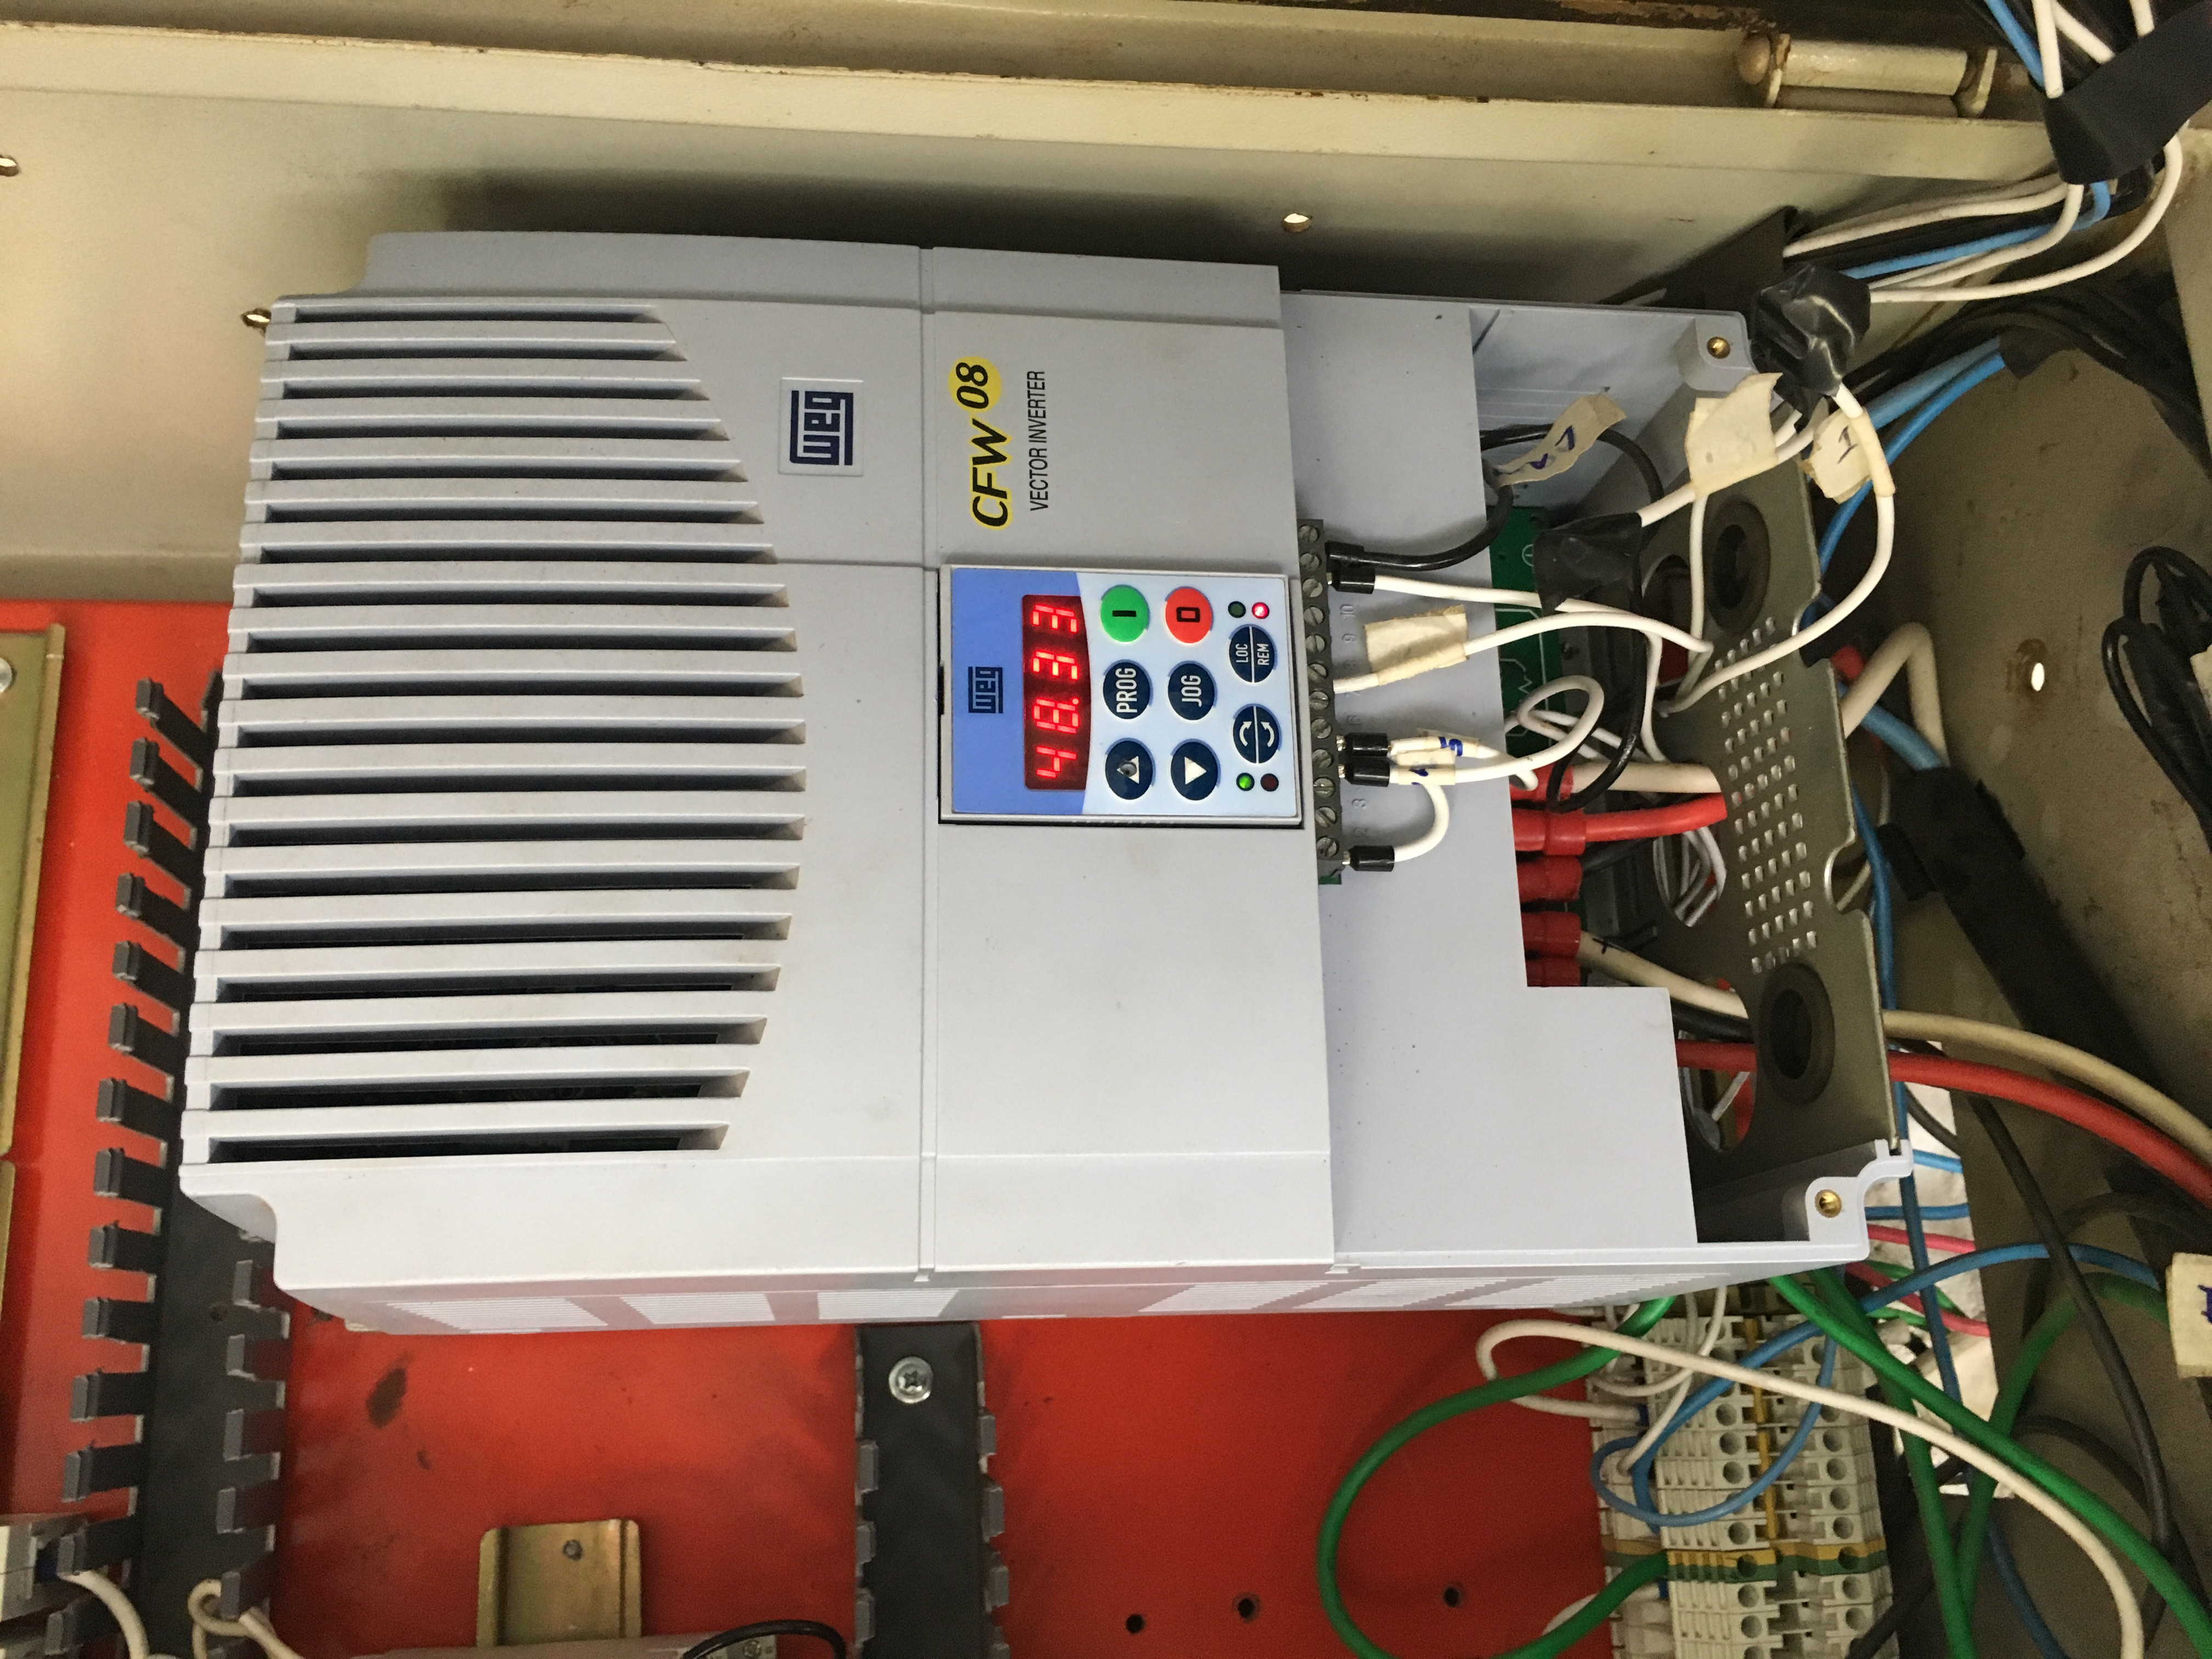
\includegraphics[scale=0.7]{figuras/fig-frequency-inverter}
			\caption{Frequency Inverter WEG-CFW08}
			\label{fig:frequency-inverter}
		\end{figure}
		\par

		The electric motor used is the WEG-xxx, this is a three-phase motor is xx cv of power (xx W) xxxx (more specs) \cite{weg-motor} and it is connected to the brake disc machine through a pulley system. Figure \ref{fig:electric-motor}.

		\begin{figure}[htbp]
			\centering
			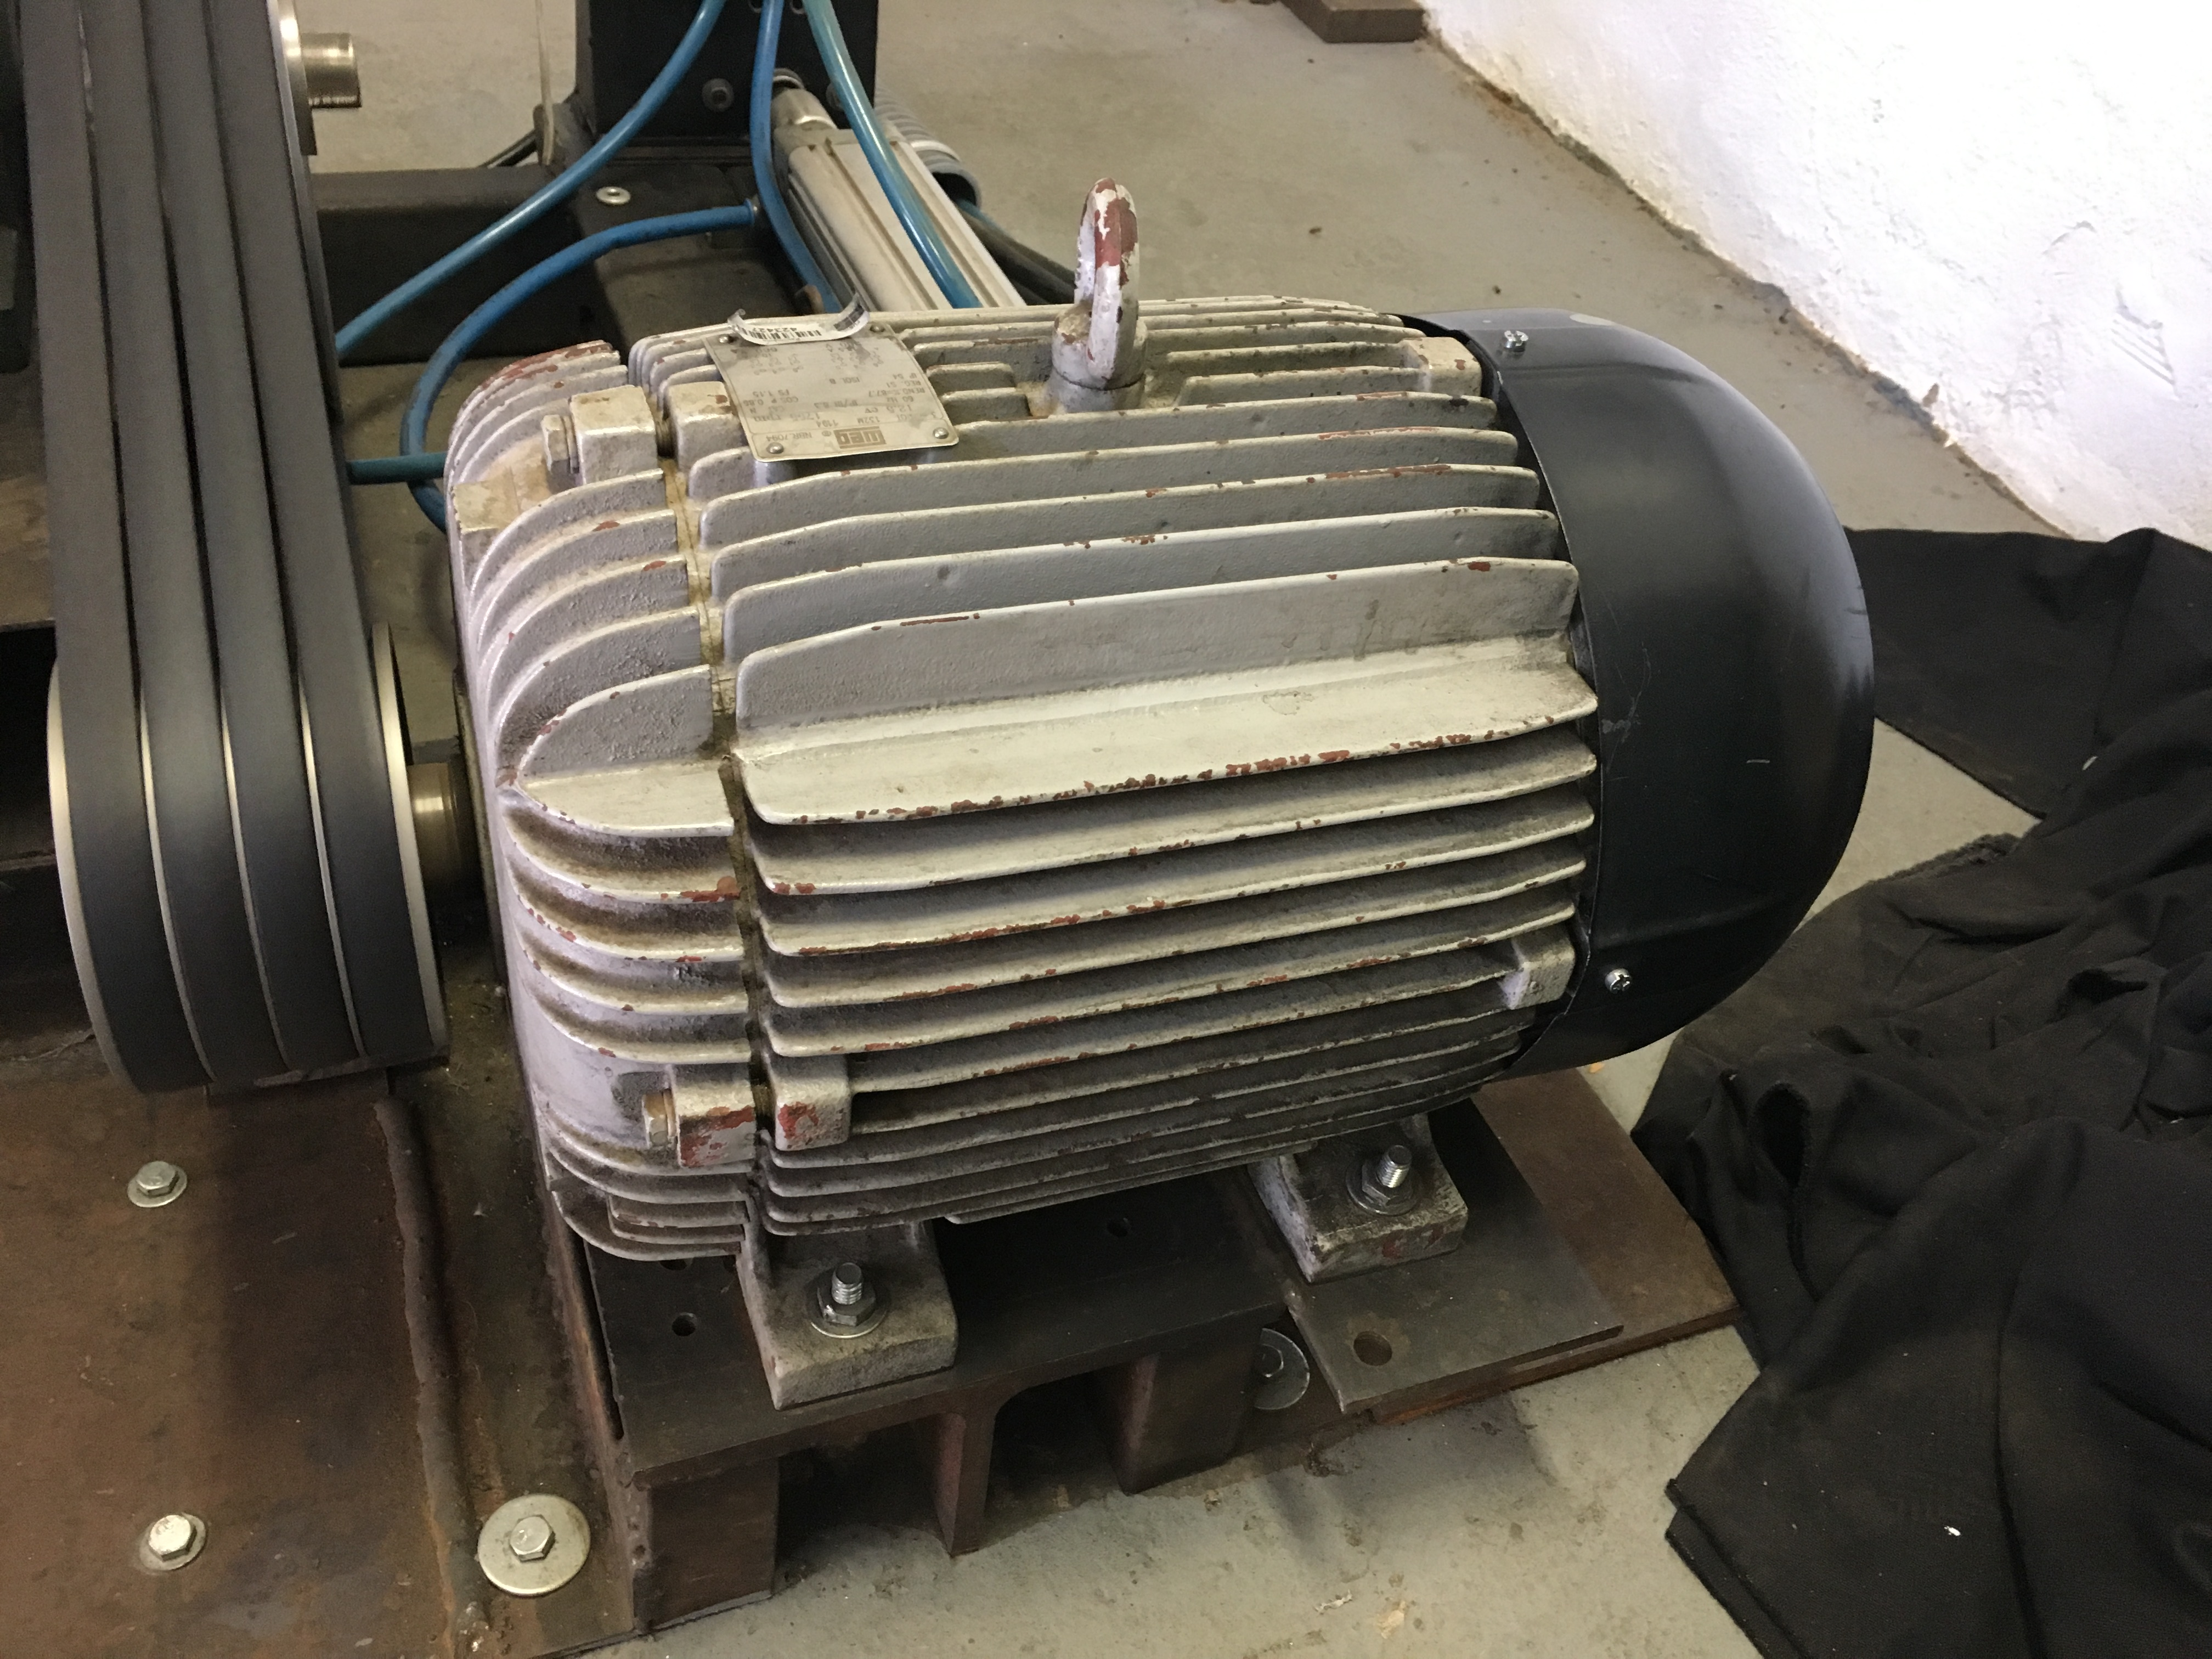
\includegraphics[scale=0.7]{figuras/fig-electric-motor}
			\caption{Frequency Inverter WEG-CFW08}
			\label{fig:electric-motor}
		\end{figure}
		\par

		Brake Disc Machine is a machine wielded on \textit{Laboratory of Automotive Engineering} in order to simulate a car's axle submitted to inertial masses. At one end the axle is connected to the electric motor through a pulley system and at the other end connected to the disc brake components as Figure \ref{fig:brake-disc-machine}.

		\begin{figure}[htbp]
			\centering
			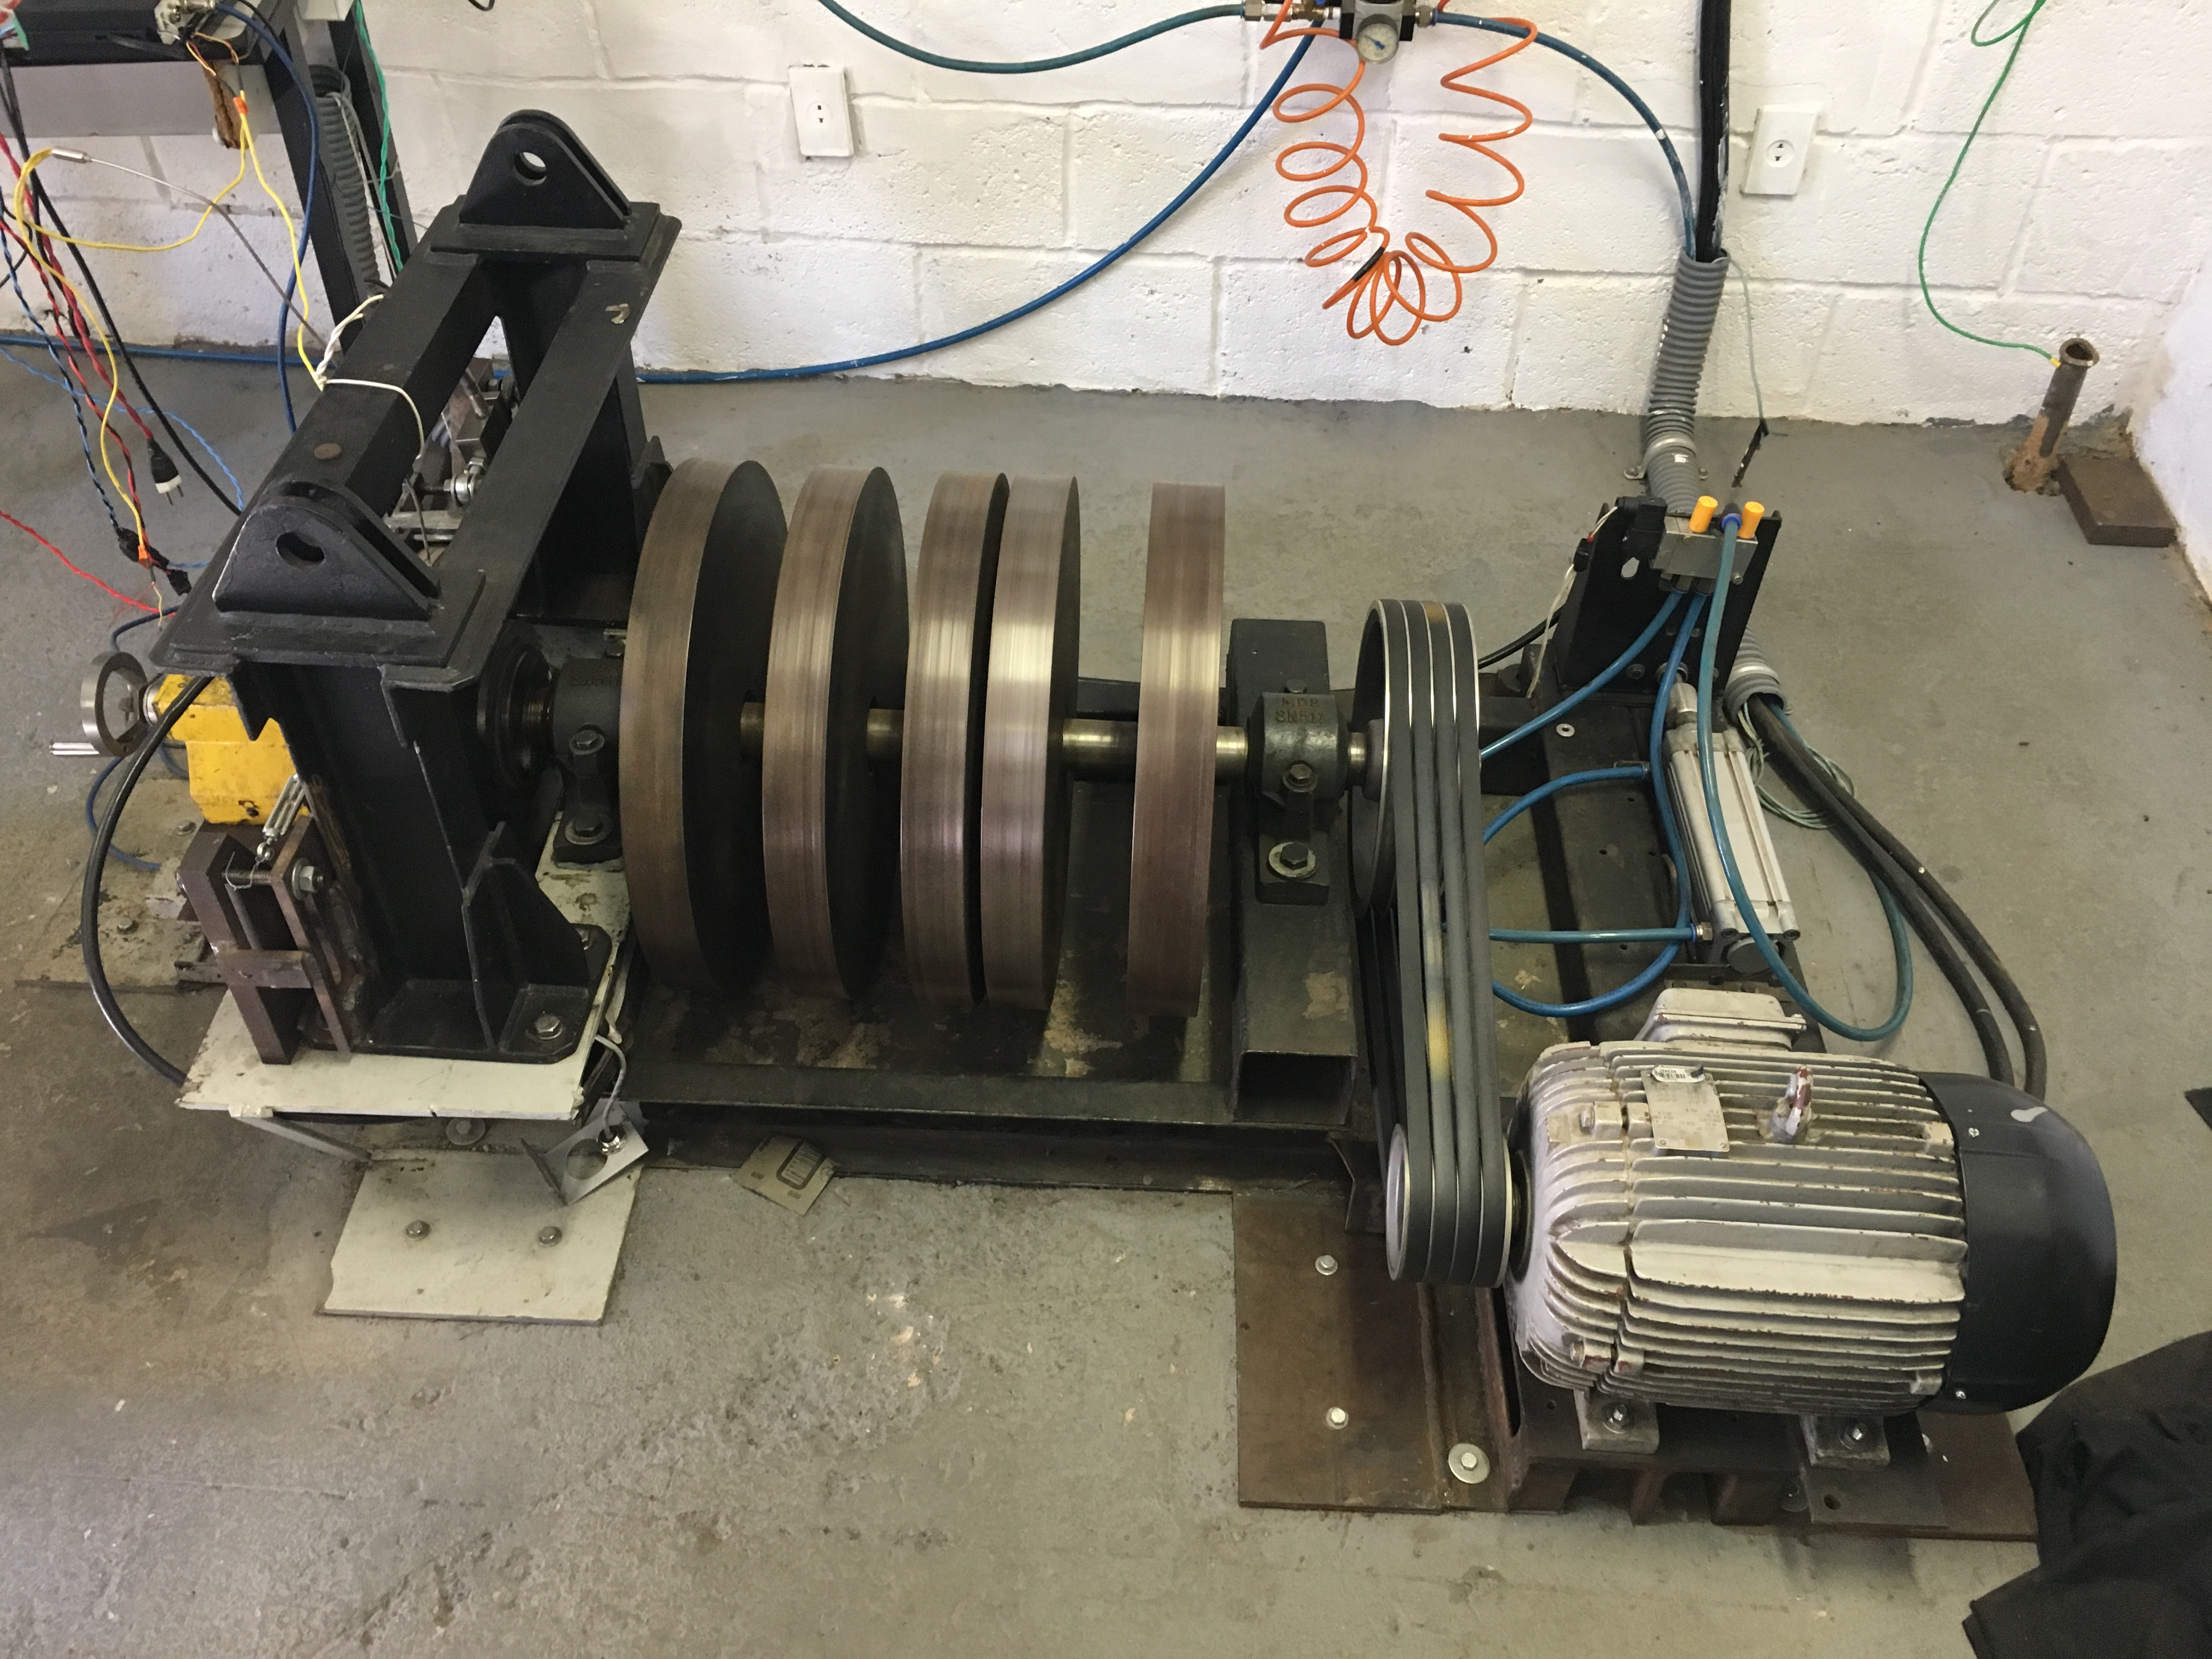
\includegraphics[scale=0.7]{figuras/fig-brake-disc-machine}
			\caption{Brake Disc Machine}
			\label{fig:brake-disc-machine}
		\end{figure}
		\par

		The Load Cell used to measure the brake force is a xxxxx from xxxx \cite{load-cell}, it has a sensibility of 2mV/V and a maximum load of 500kgf, meaning when it is powered with 2V5 (check Section \ref{ssec:load-cell-signal-conditioning}) and submitted to its maximum load the voltage output will be of 5V. Figure \ref{fig:load-cell-installation-scheme} shows how the load cell can be used to measured the braking force and Figure \ref{fig:load-cell-installed} shows the actual load cell installed on the Brake Disc Machine.

		\begin{figure}[htbp]
			\centering
			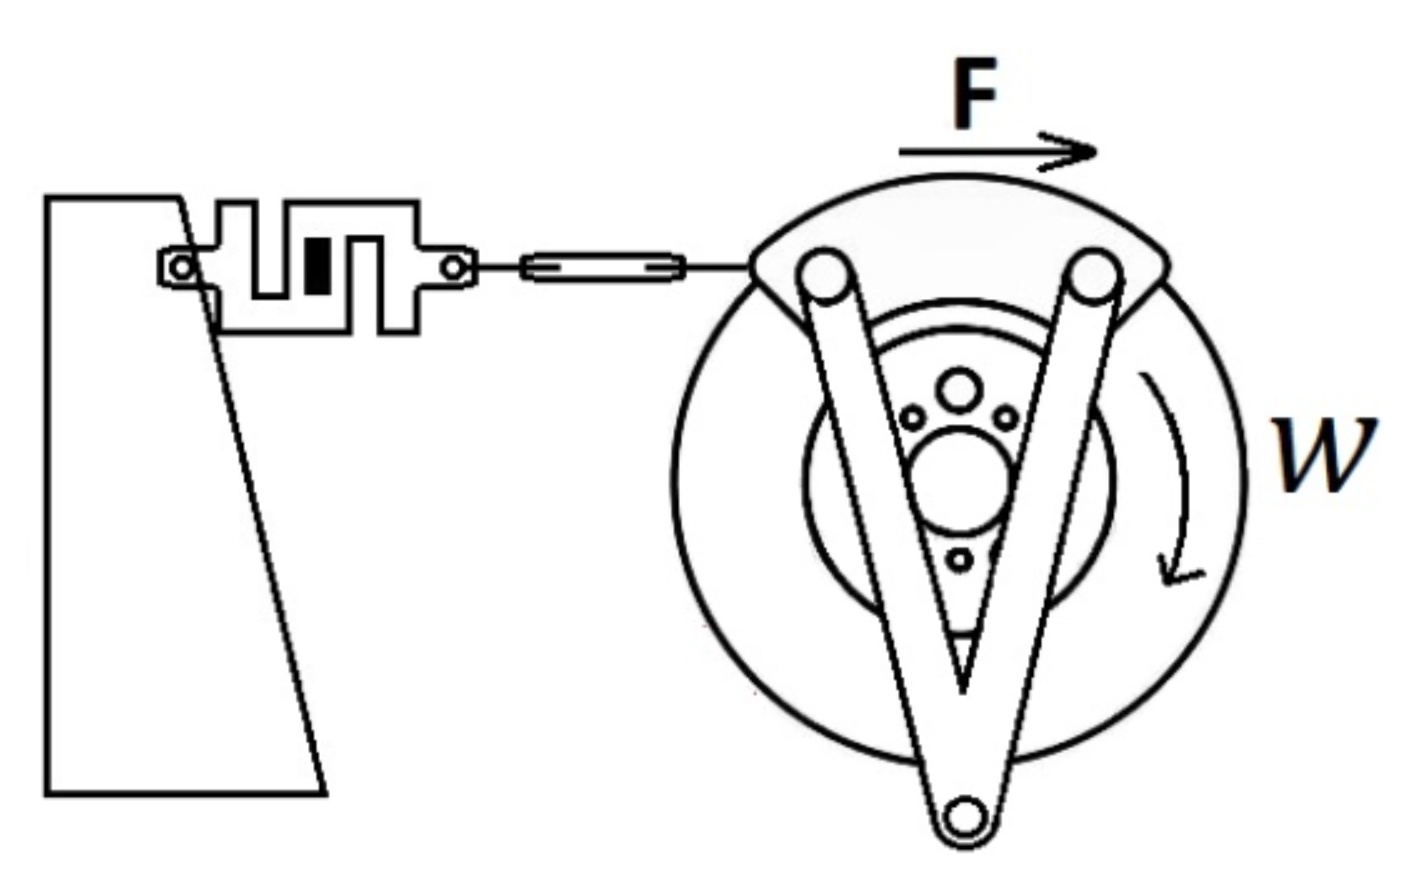
\includegraphics[scale=0.7]{figuras/fig-load-cell-installation-scheme}
			\caption{Load Cell Installation Scheme \cite{load-cell-caxeta2017}}
			\label{fig:load-cell-installation-scheme}
		\end{figure}

		\begin{figure}[htbp]
			\centering
			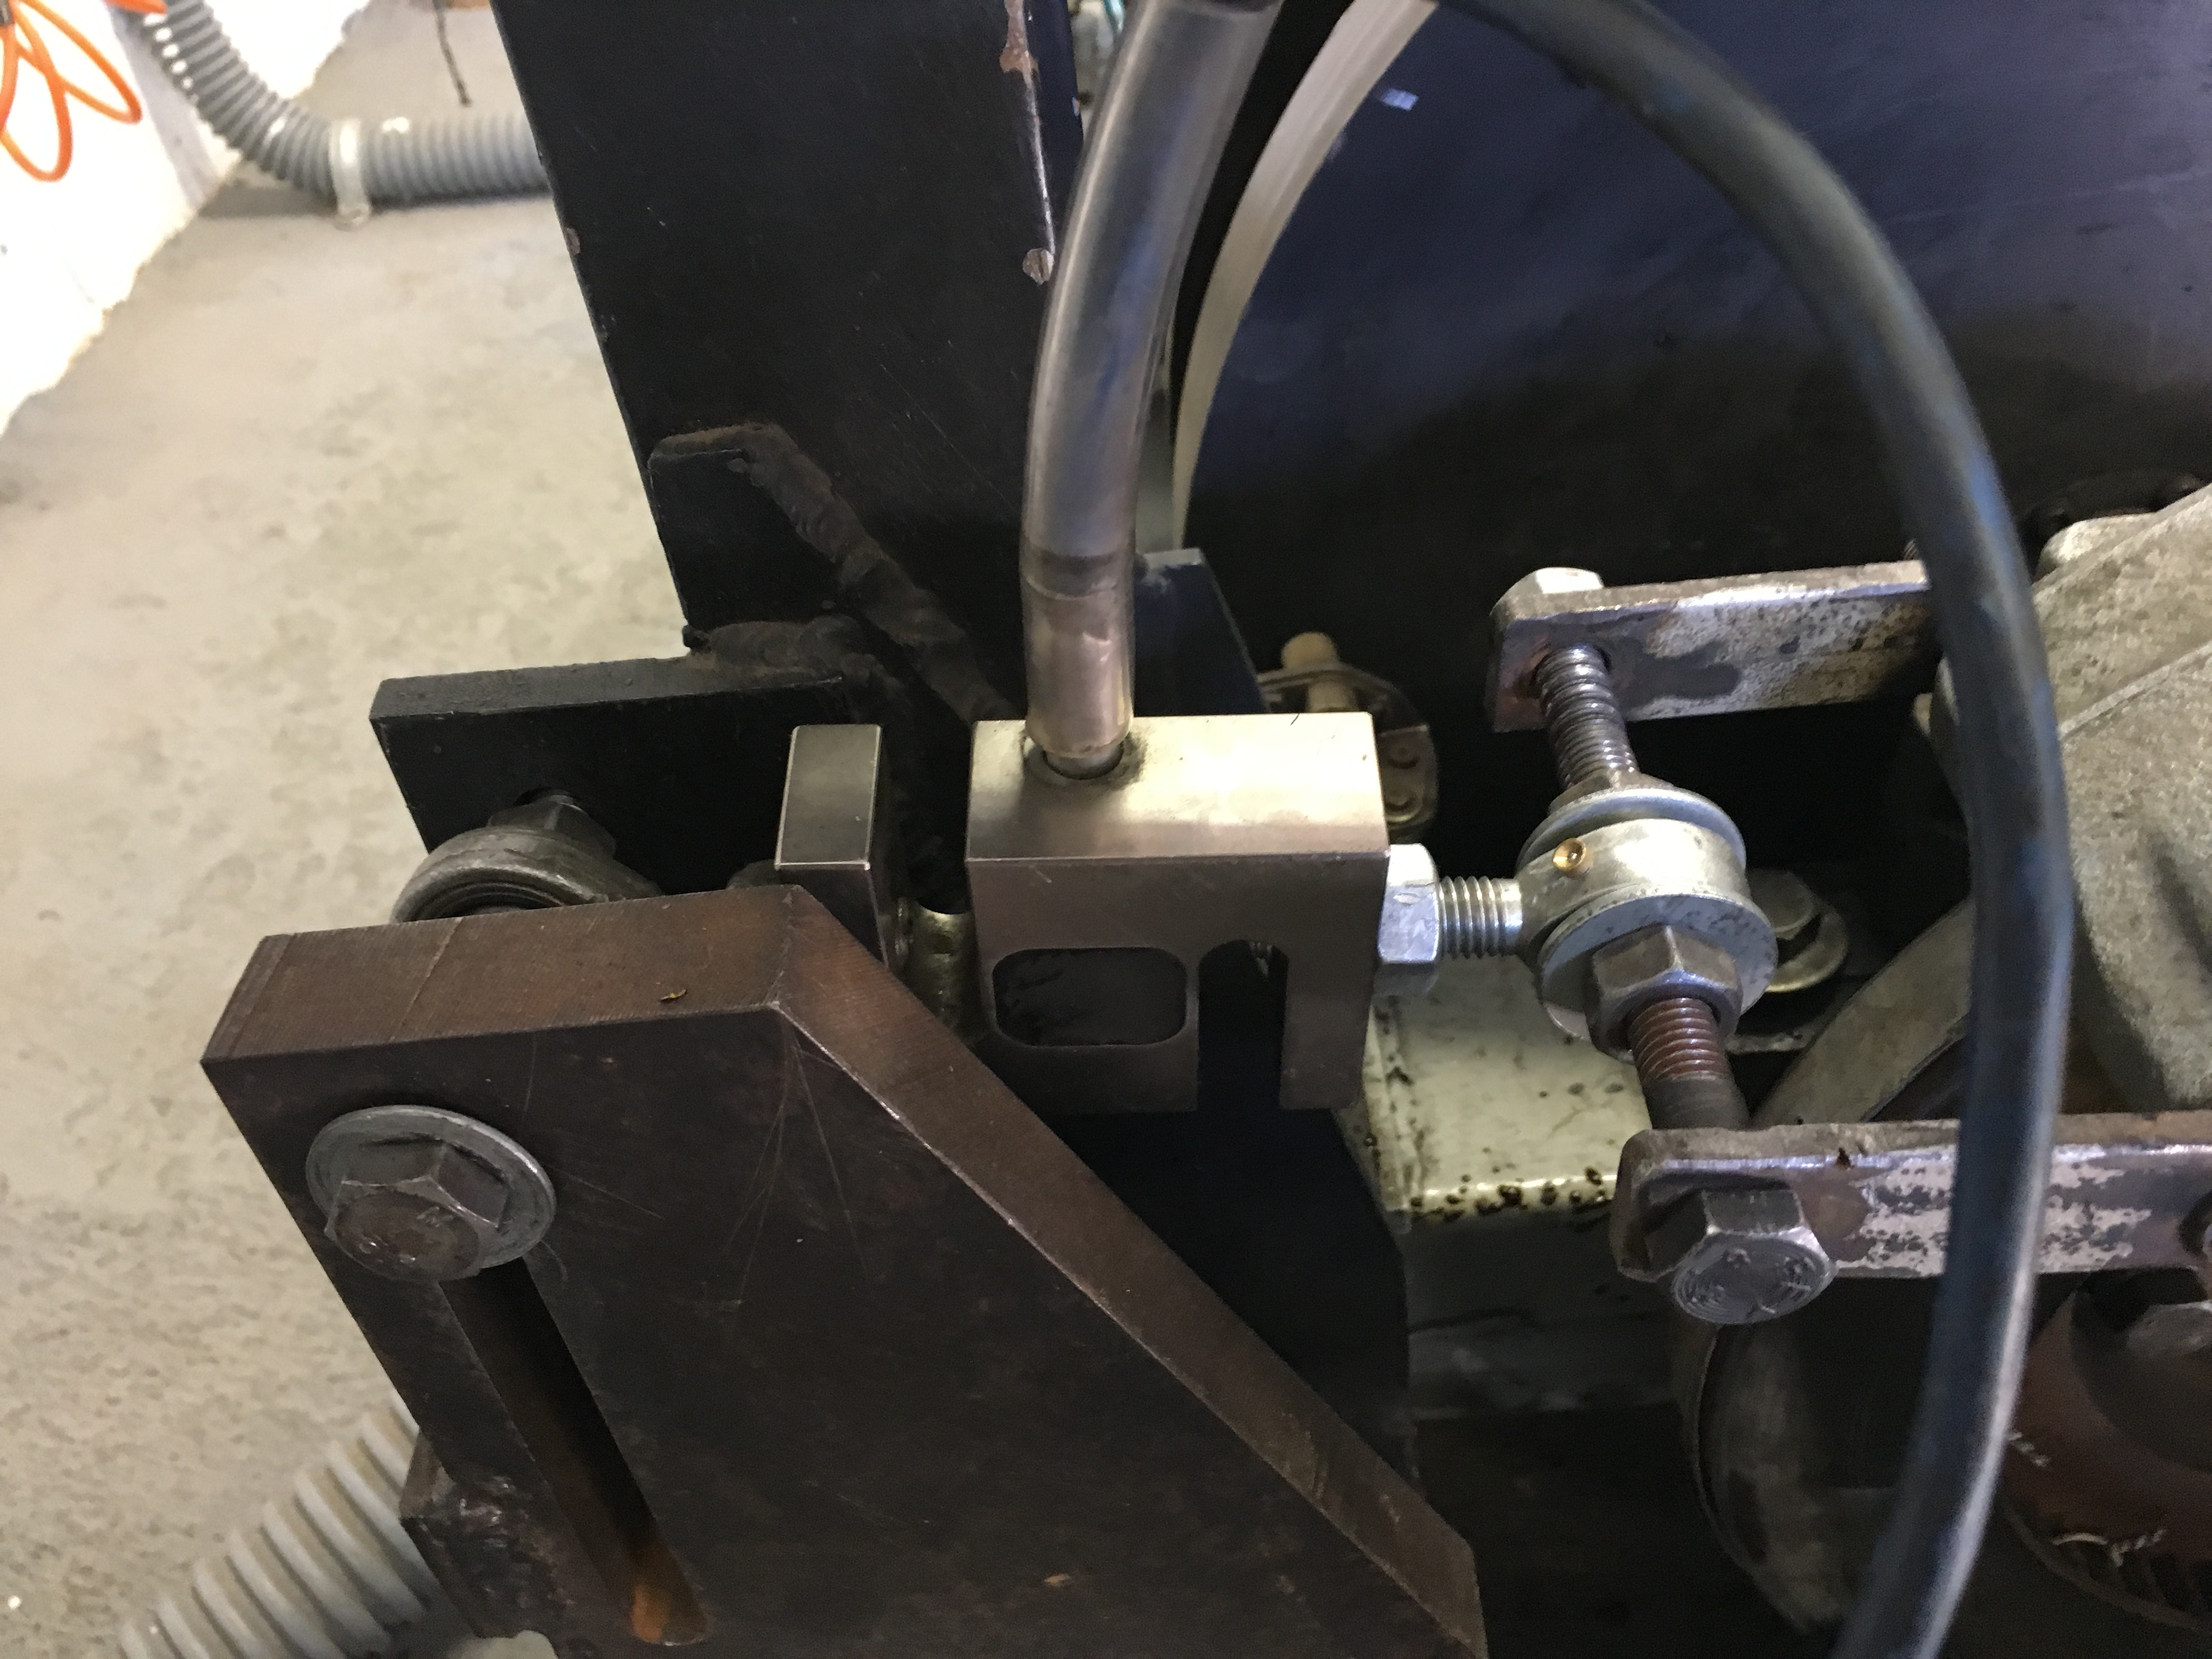
\includegraphics[scale=0.7]{figuras/fig-load-cell-installed}
			\caption{Load Cell Installed}
			\label{fig:load-cell-installed}
		\end{figure}
		\par

		This project uses two generic type K themocouples at each end of the braking disc, as Figure \ref{fig:thermocouple-installation} shows.

		\begin{figure}[htbp]
			\centering
			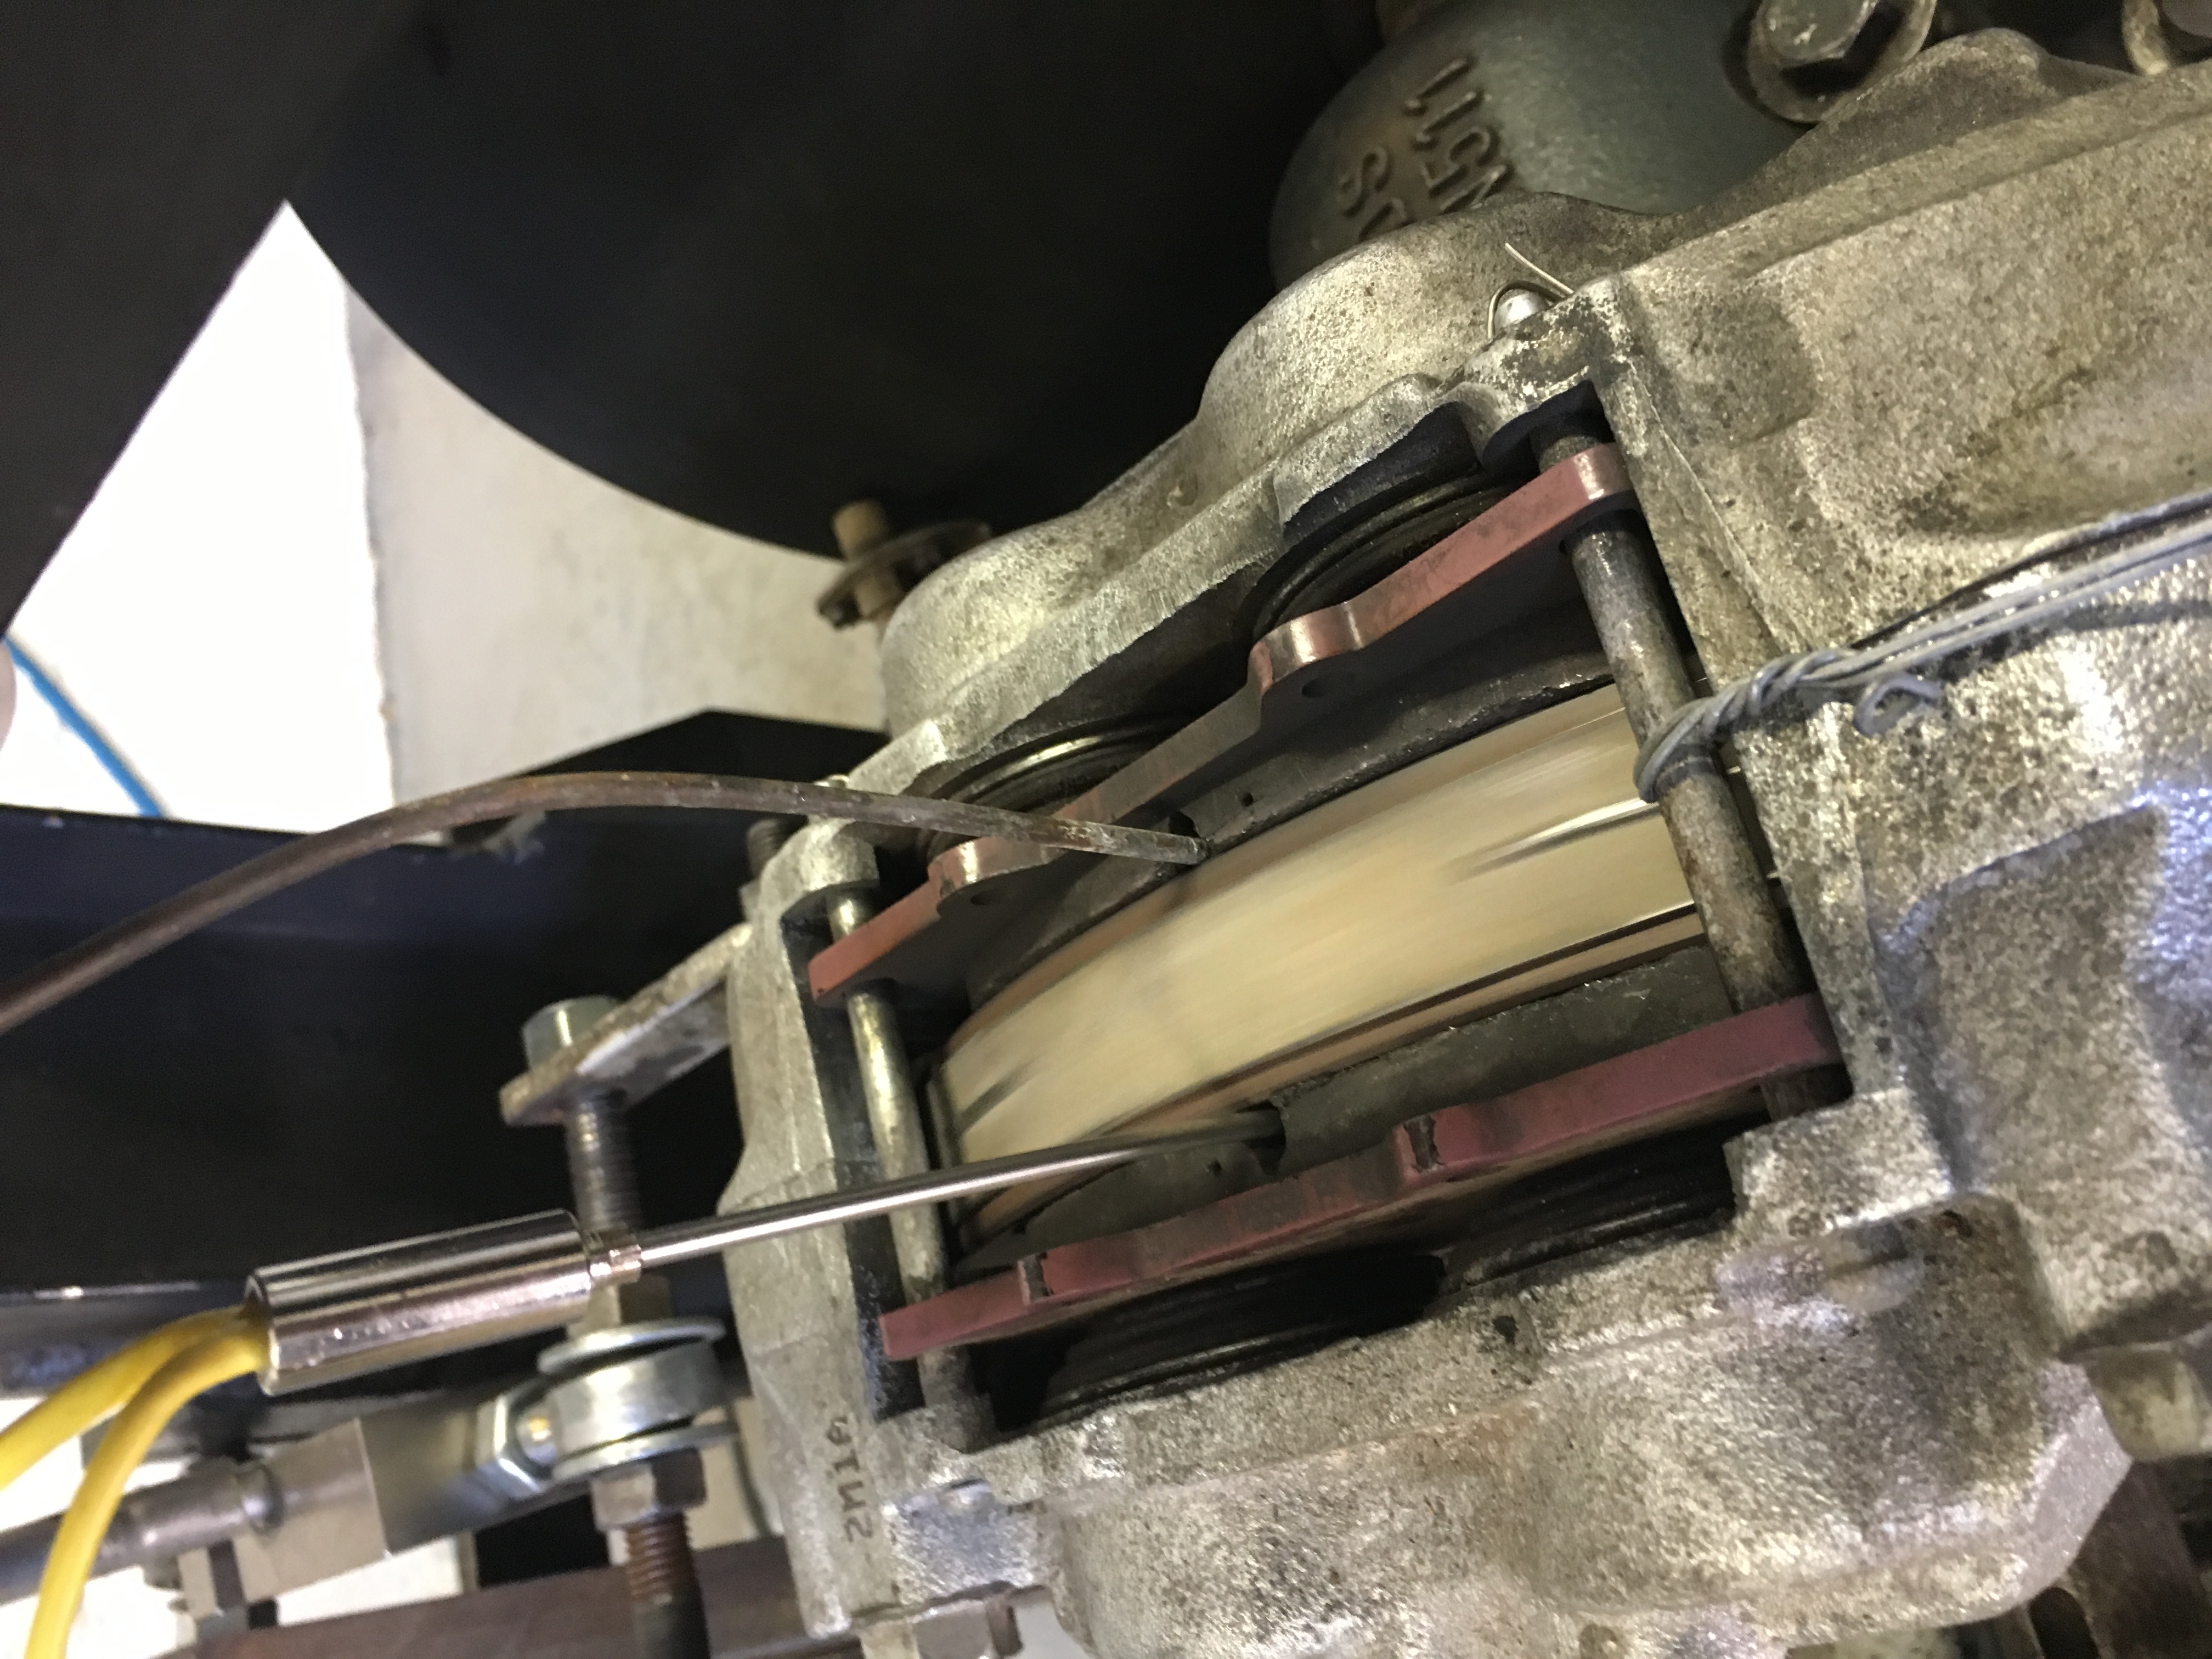
\includegraphics[scale=0.7]{figuras/fig-thermocouple-installation}
			\caption{Thermocouples Installed}
			\label{fig:thermocouple-installation}
		\end{figure}
		\par

		This project also includes a generic Crankshaft Position Sensor, to enhance the CKP signal amplitude six small magnets were placed around the inertial disc that the CKP is perpendicular mounted to, the only important consideration when doing this is that the CKP will actualy measure a frequency six times higher than the actual rotation frequency of the axel. Figures \ref{fig:inertial-mass-with-magnets} and \ref{fig:ckp-installed} shows how the magnets and the CKP sensor was placed.

		\begin{figure}[htbp]
			\centering
			\includegraphics[scale=0.7]{figuras/fig-inertial-mass-with-magnets}
			\caption{Innertial mass with magnets placed}
			\label{fig:inertial-mass-with-magnets}
		\end{figure}

		\begin{figure}[htbp]
			\centering
			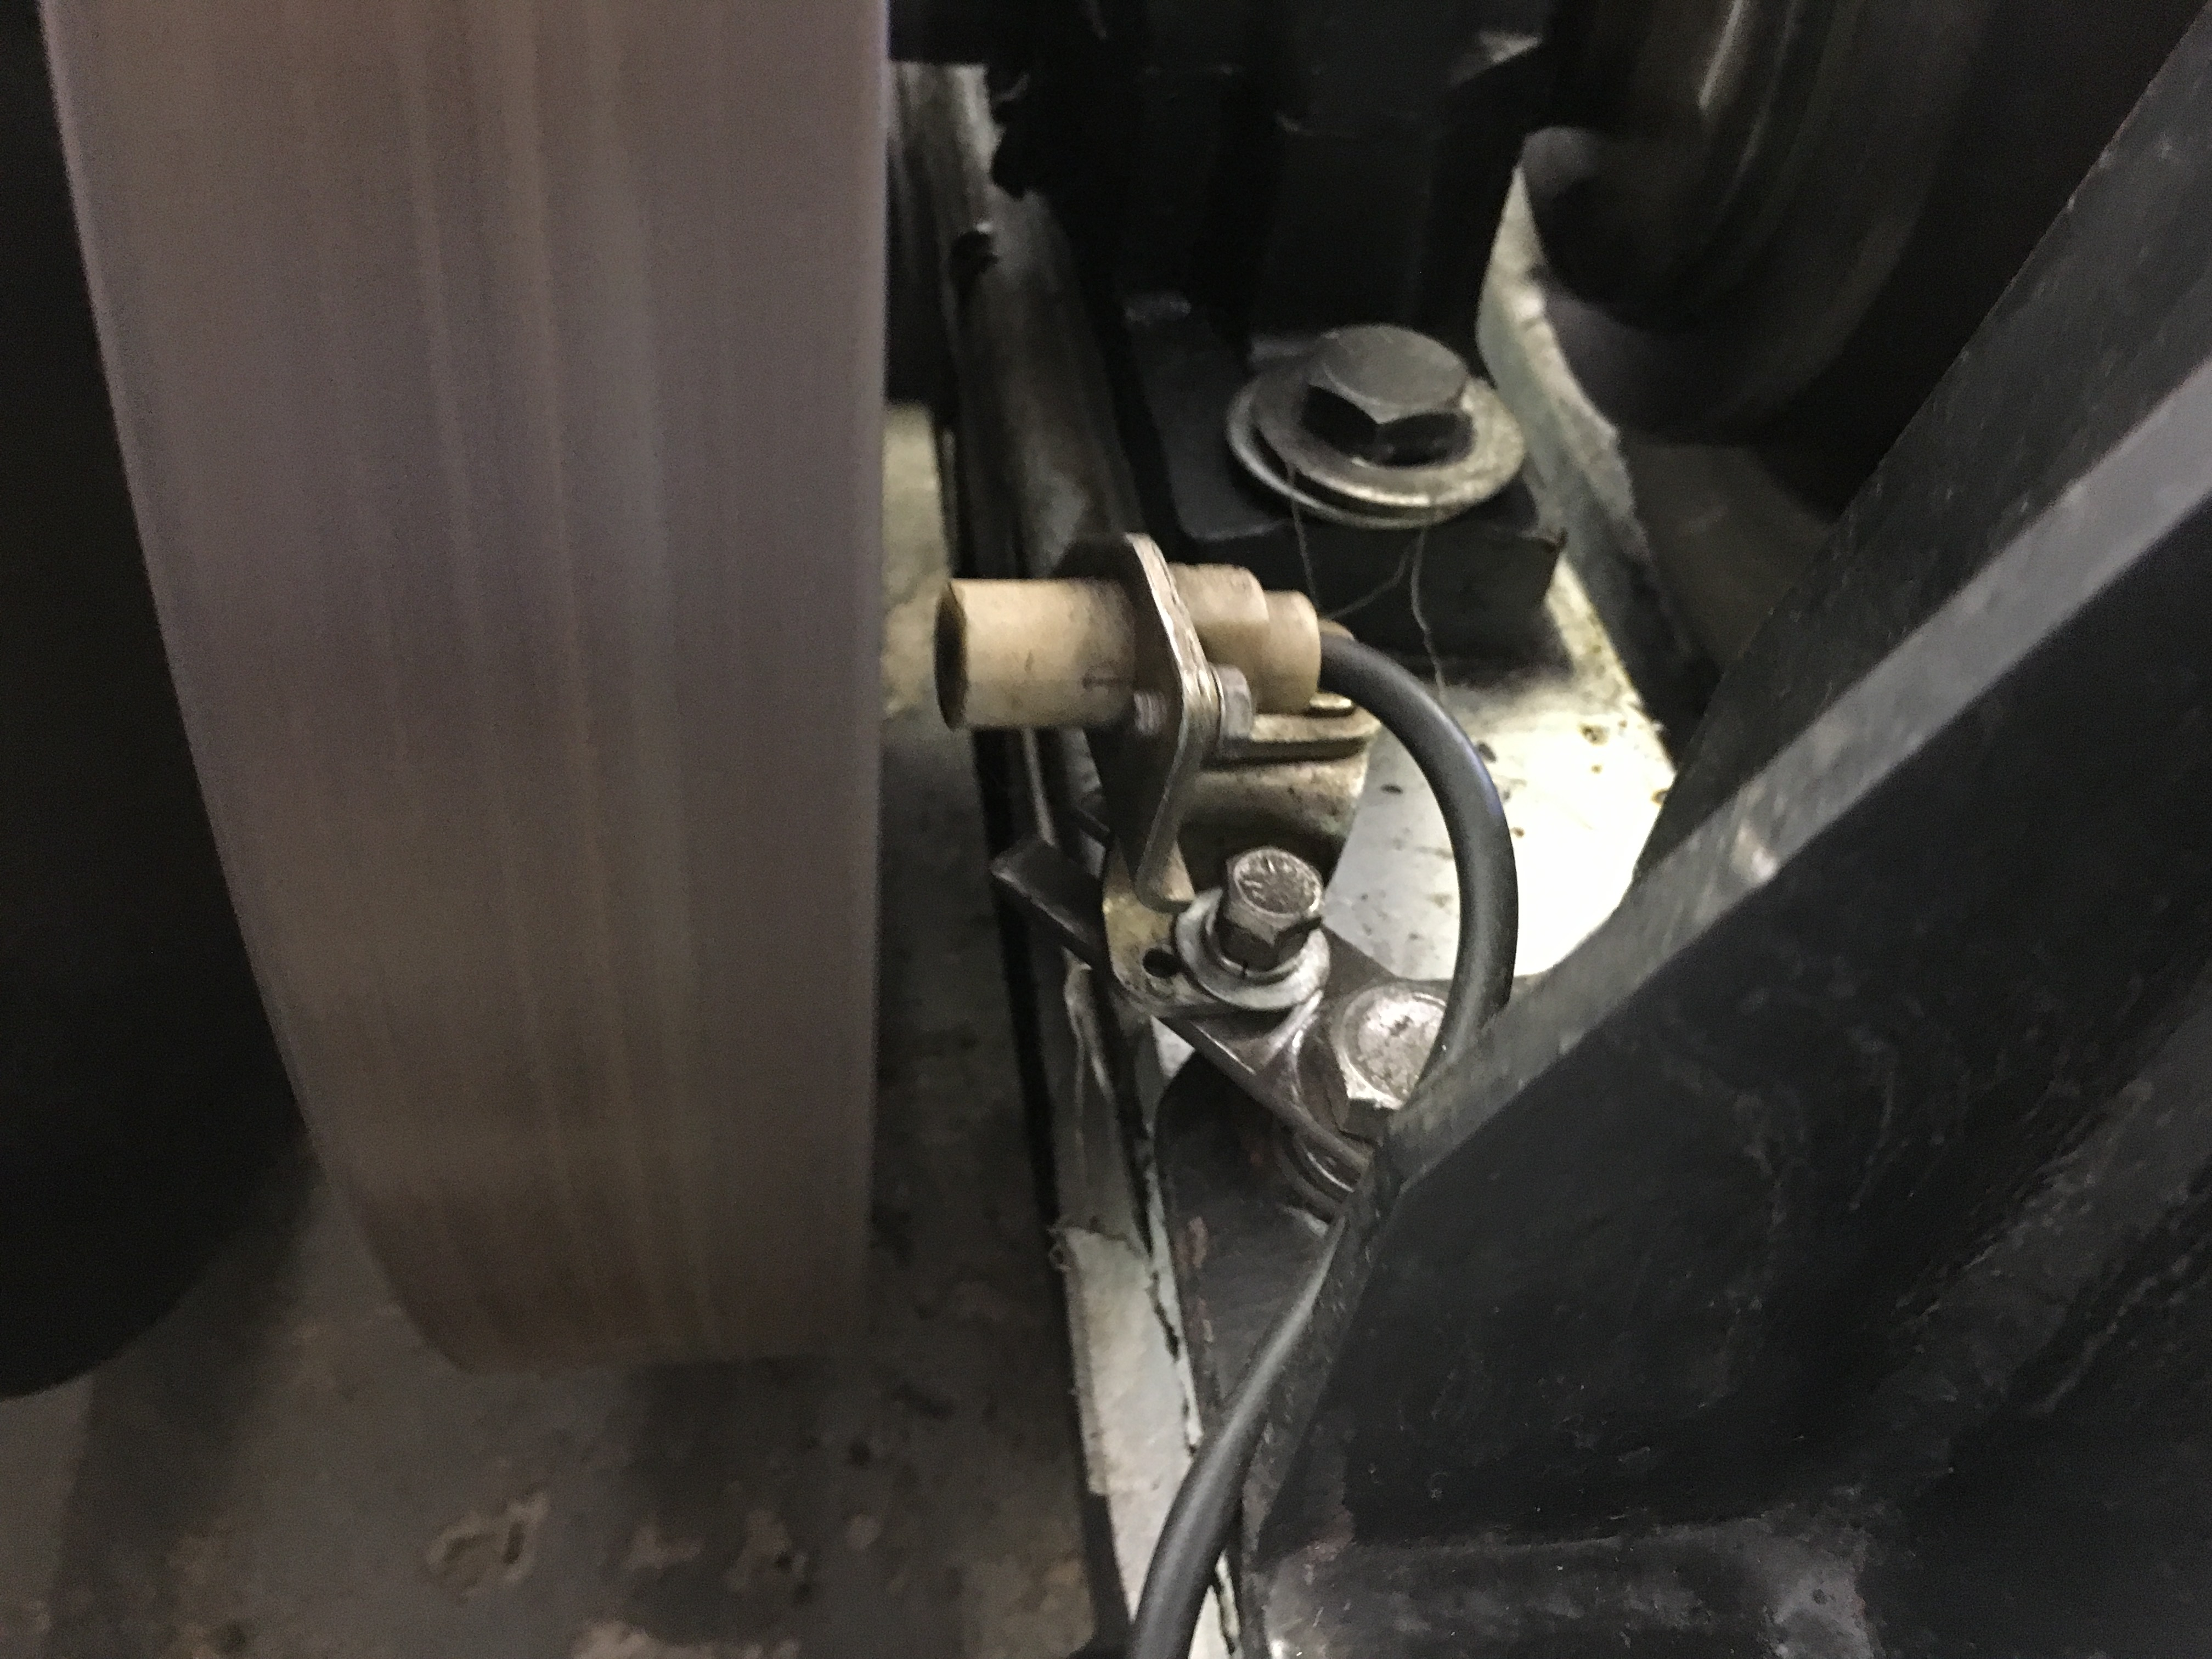
\includegraphics[scale=0.7]{figuras/fig-ckp-installed}
			\caption{CKP installed}
			\label{fig:ckp-installed}
		\end{figure}
		\par

		Additional materials used for the test are the developed hardware and the laptop used to run the test.
		\section{Test Application}\label{ssec:testApplication}
	In order to perform the test a \textit{LabView} application was developed to control the lower level hardware and perform data processing, the application main screen can be seen in Figure \ref{fig:labview-app-mainscreen}.

	\begin{figure}[htbp]
		\centering
		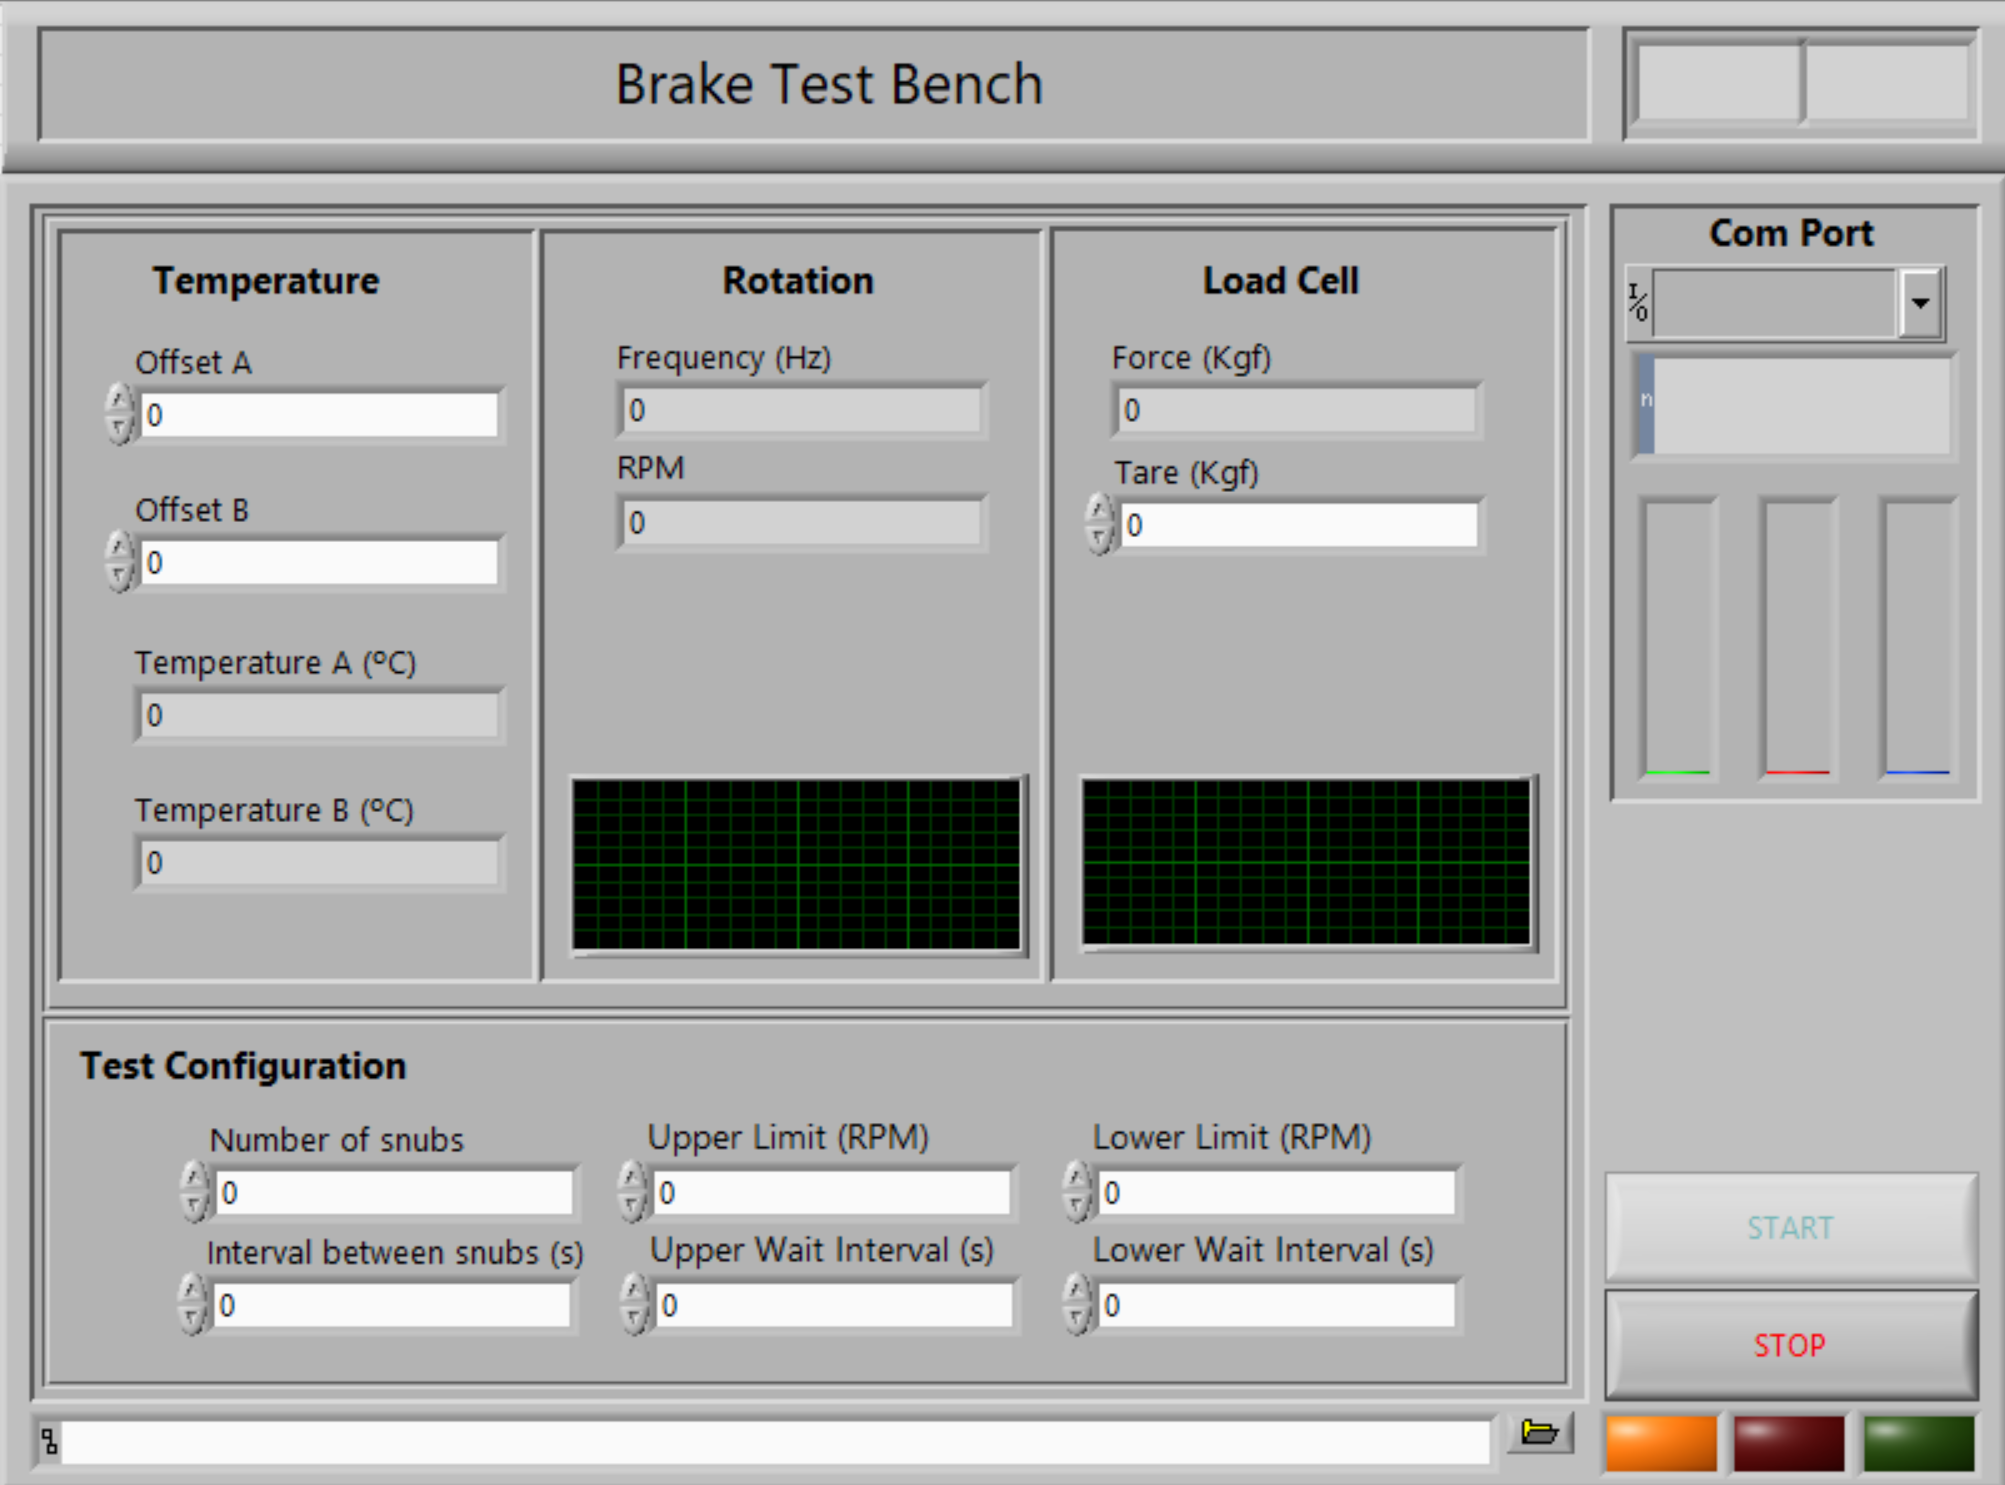
\includegraphics[width=.8\textwidth]{figuras/fig-labview-app-mainscreen}
		\caption{Test Application Main Screen}
		\label{fig:labview-app-mainscreen}
	\end{figure}

	The main screen is divided in three parts, first part displays the sensors readings, thermocouples measured temperature, rotation frequency and RPMs and load cell braking force. On the bottom of the screen the test configurations, them being:

	\begin{itemize}
		\item\textit{Number of Snubs:} The number of times each brake iteraction will be done.
		\item\textit{Interval between snubs (s):} The amount of seconds that a interface will wait at the end of a brake iteraction before accelerating the motor again.
		\item\textit{Upper Limit (RPM):} At each snub the system will accelerate the electric engine until the rotor reaches this pre-defined rotation rhythm.
		\item\textit{Upper Wait Interval (s):} After reaching the upper rotation limit the system will wait for this interval before braking.
		\item\textit{Lower Limit (RPM):} The system will perform braking until the rotor reaches this lower RPM limit.
		\item\textit{Lower Wait Interval (s):} After reaching the Lower Limit the system will for this interval.
	\end{itemize}

	The software itself will take full control of the test, it will turn the electric motor on when needed, turn the brakes one
		\section{Brake Test}\label{sec:brakeTest}

	\subsection{Full Stop Test}

	The desired test will be the full stop test, described by \cite{caixeta2017} as a test where the speed is set to a upper limit and then to nought rotation at the end. The test can also be carried with different braking pressure (different pressures at the hydraulic valve) in order to achieve more relevant data.

	\par
	In order to start the brake test the following parameters were configured on the \textit{Labview} Test Application:

	\begin{itemize}Number of Snubs: 
		\item\textit{Number of Snubs:} In order to achieve solid results, 50 snubs were set.
		\item\textit{Interval between snubs (s):} In order to let the brake pads cool, five seconds were set between each snub.
		\item\textit{Upper Limit (RPM):} The upper limit was set at 600 RPMs, that is almost the fastest measured rotation that the brake machine can achieve.
		\item\textit{Upper Wait Interval (s):} Three seconds, just enough so that the speed can stabilize.
		\item\textit{Lower Limit (RPM):} Npught, the idea is to fully stop the system.
		\item\textit{Lower Wait Interval (s):} Nought, as the \textit{Lower Limit (RPM)} will be zero, this time can be compreheended inside the \textit{Inverval Between Snubs}.
	\end{itemize}

	The test shall be carried twice, first with 1000kPa and later with 200kPa in order to compare results. The goal of this tests is not to evaluate braking performance of components of a brake system but rather to prove that the developed hardware can be used for that, i.e. showing that the measured quantities are directly related to the tests are being carried out. Hence, temperature should increase after each snub, the measured braking pressure should increase as the braking actuator is activated and the CKP signal frequency should start increasing shortly after the electric motor is turned on.

	\subsection{Results}

	Figure \ref{fig:1000k-braking-test-graph} shows the results for the test with 1000kPa...